\section{Appendix}
\subsection{Baseline measurements C++}

\begin{figure}[!htbp]
  \centering
  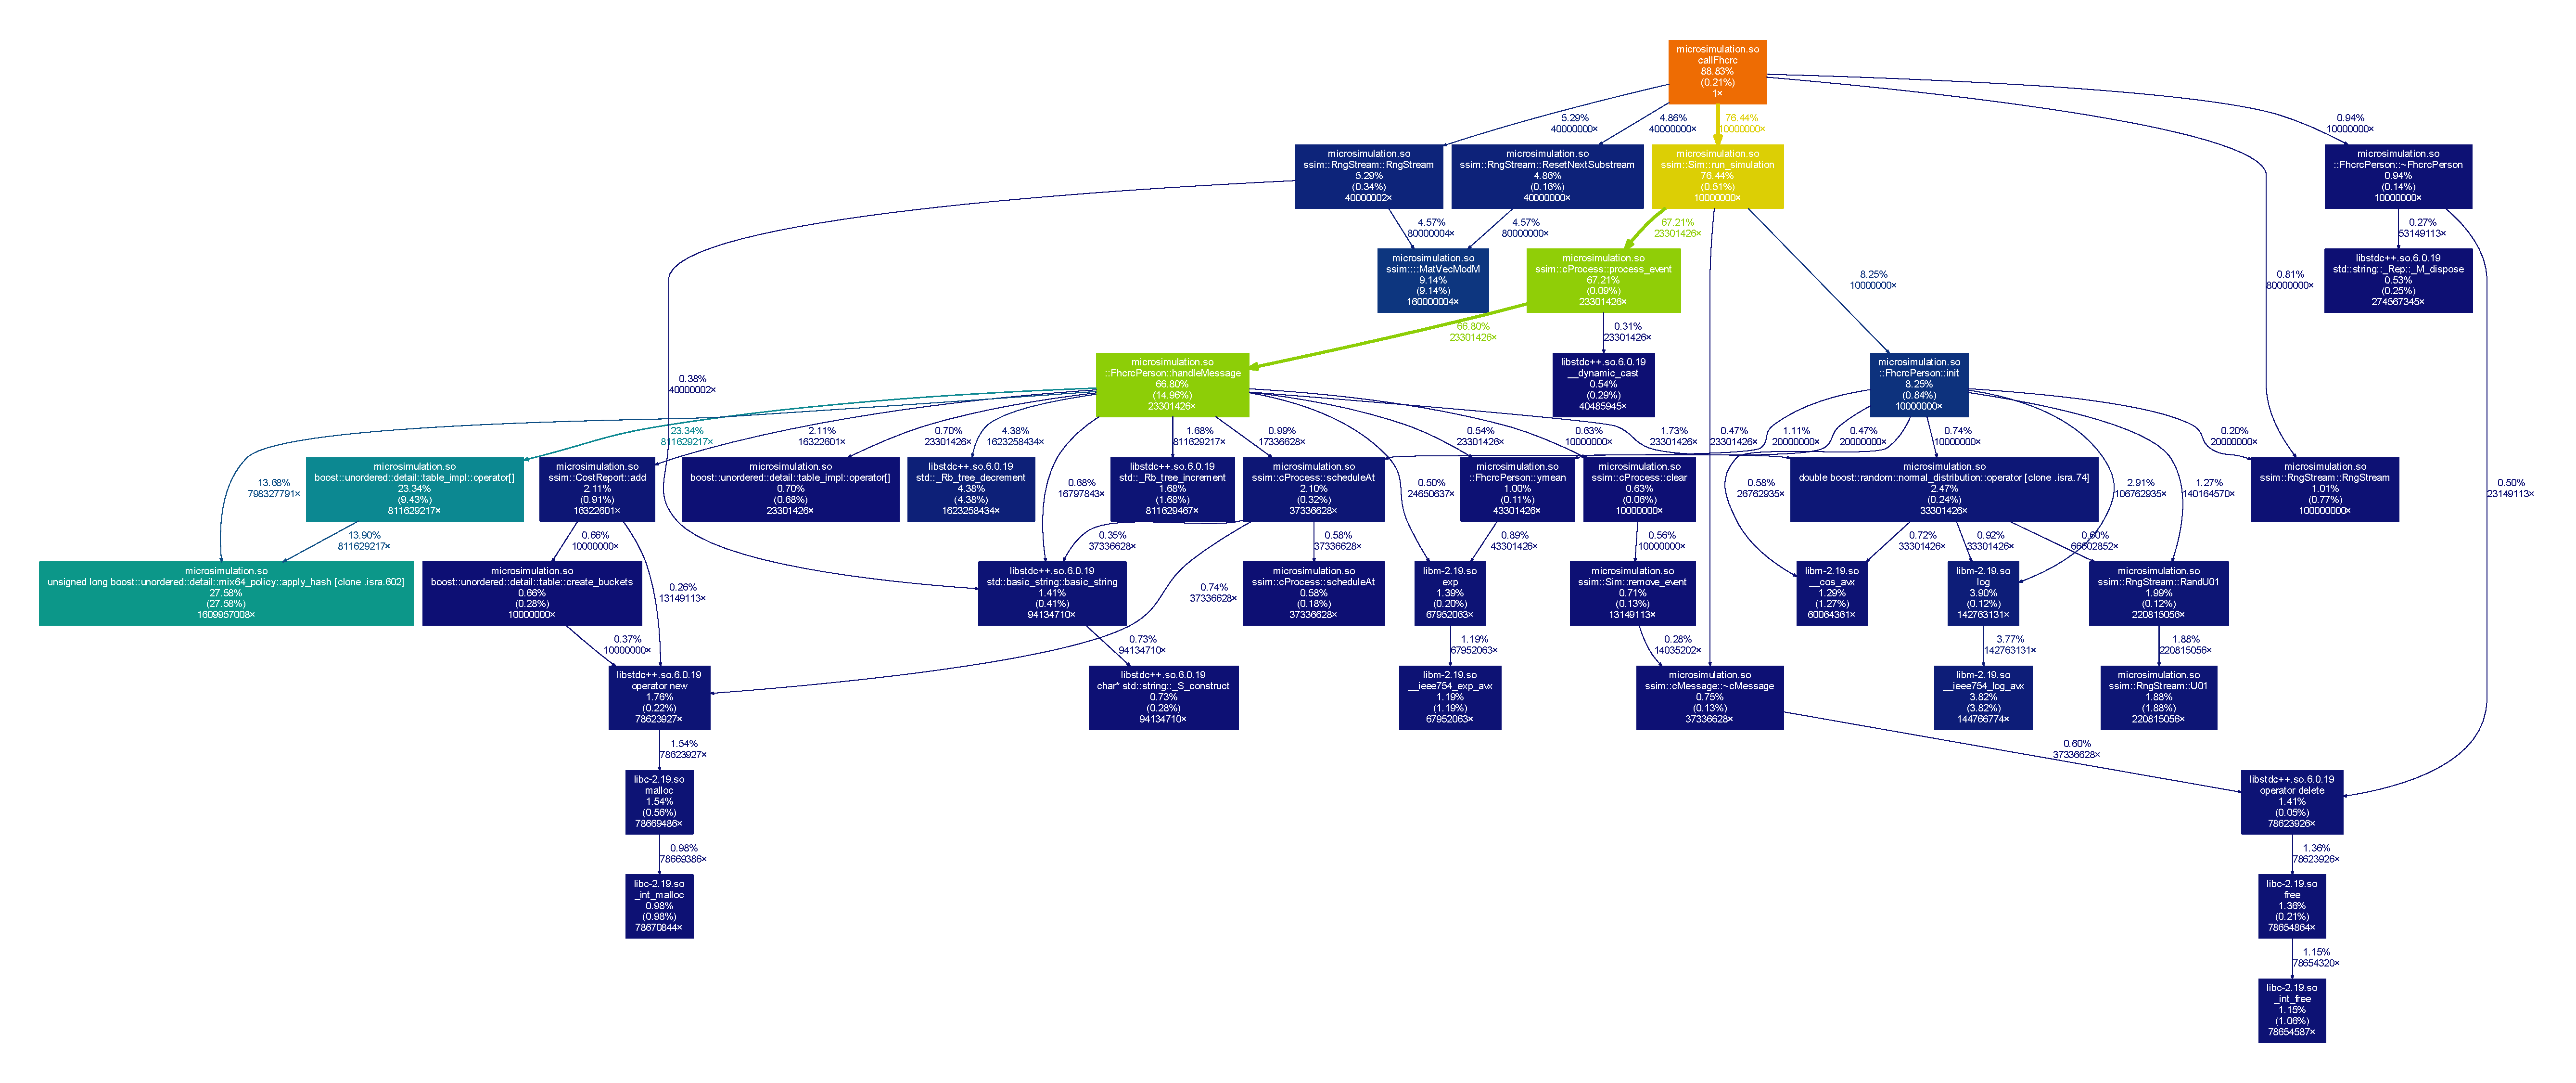
\includegraphics[height=0.50\textheight, angle=90]{images/profBaseLine.pdf}
  \caption{Valgrind measurements at baseline}
  \label{fig:baseline}
\end{figure}


\subsection{Simple approach with OpenMP}
\begin{figure}[!htbp]
  \centering
  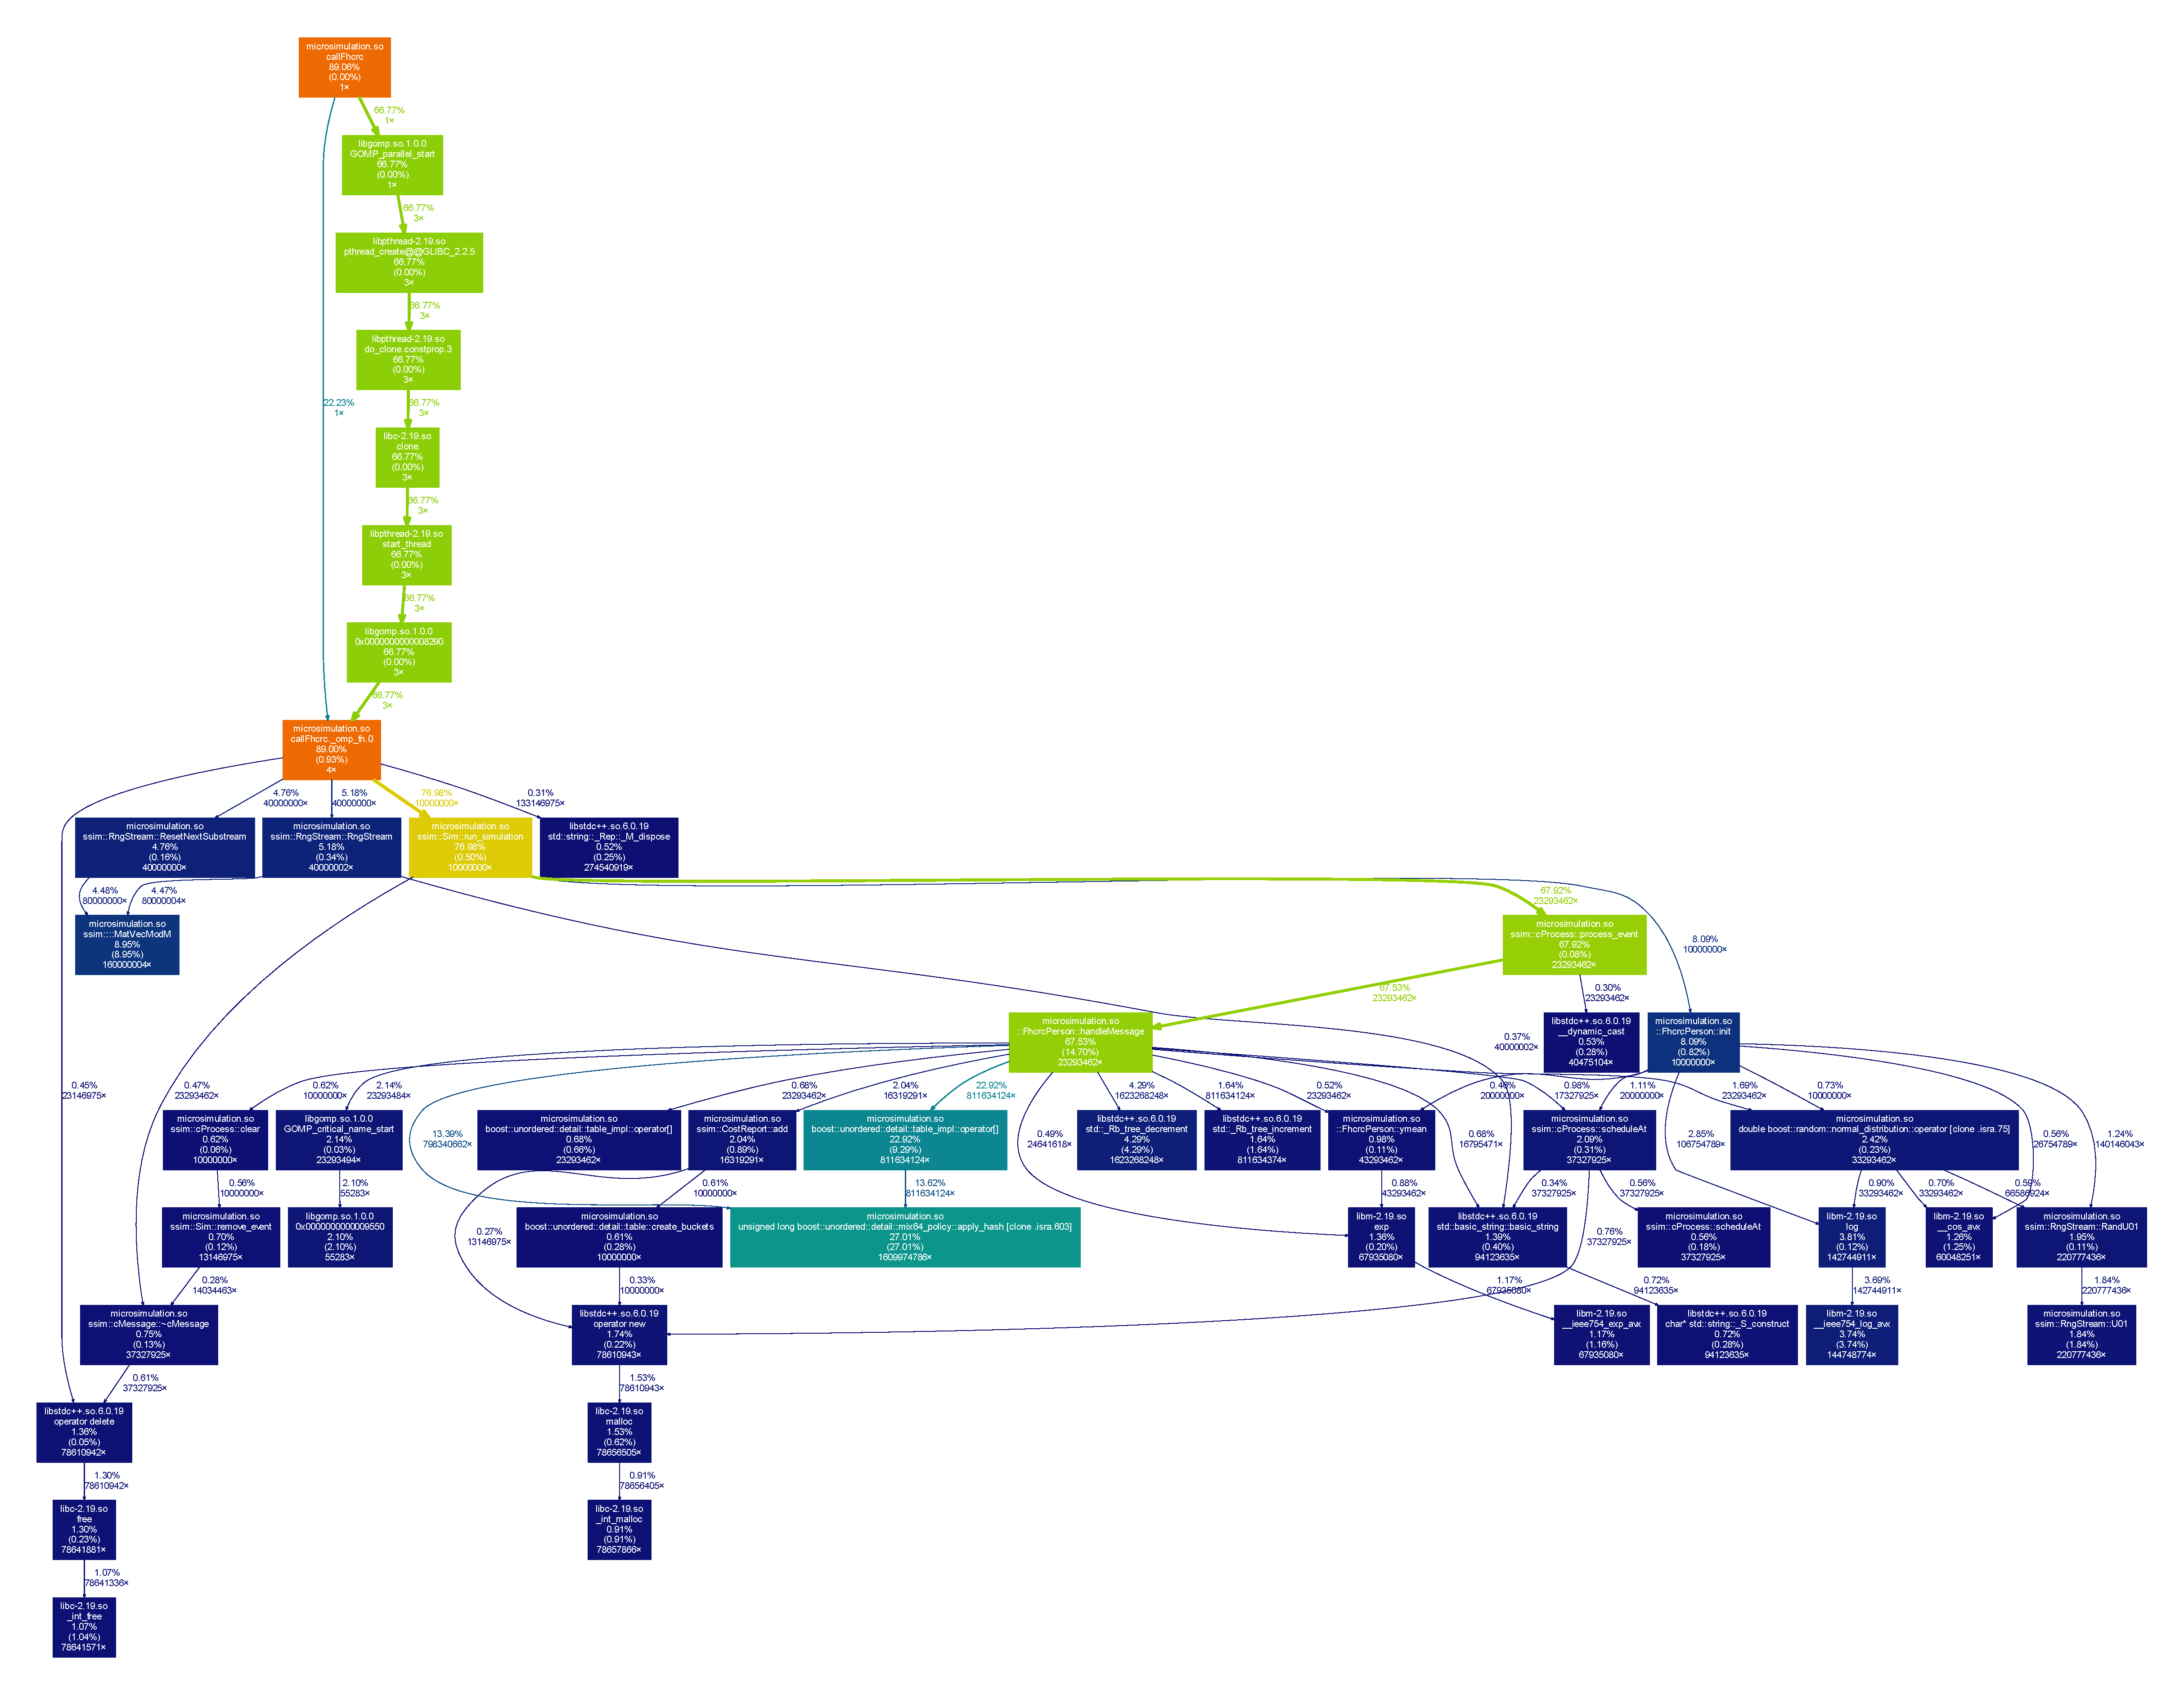
\includegraphics[height=0.85\textheight, angle=90]{images/profOpenMPSimple.pdf}
  \caption{Valgrind results of the naive openMP implementation}
  \label{fig:naiveOpenMP}
\end{figure}

Here the simulation loop is run in parallel whereas the data output
and some post-processing is run within a omp critical statement.


%%% Local Variables:
%%% mode: latex
%%% TeX-master: "report"
